\section{Architettura}
L'architettura realizzata è presentata in figura \ref{img:architecture}.

\begin{figure}[!ht]
\begin{center}
\makebox[\linewidth]{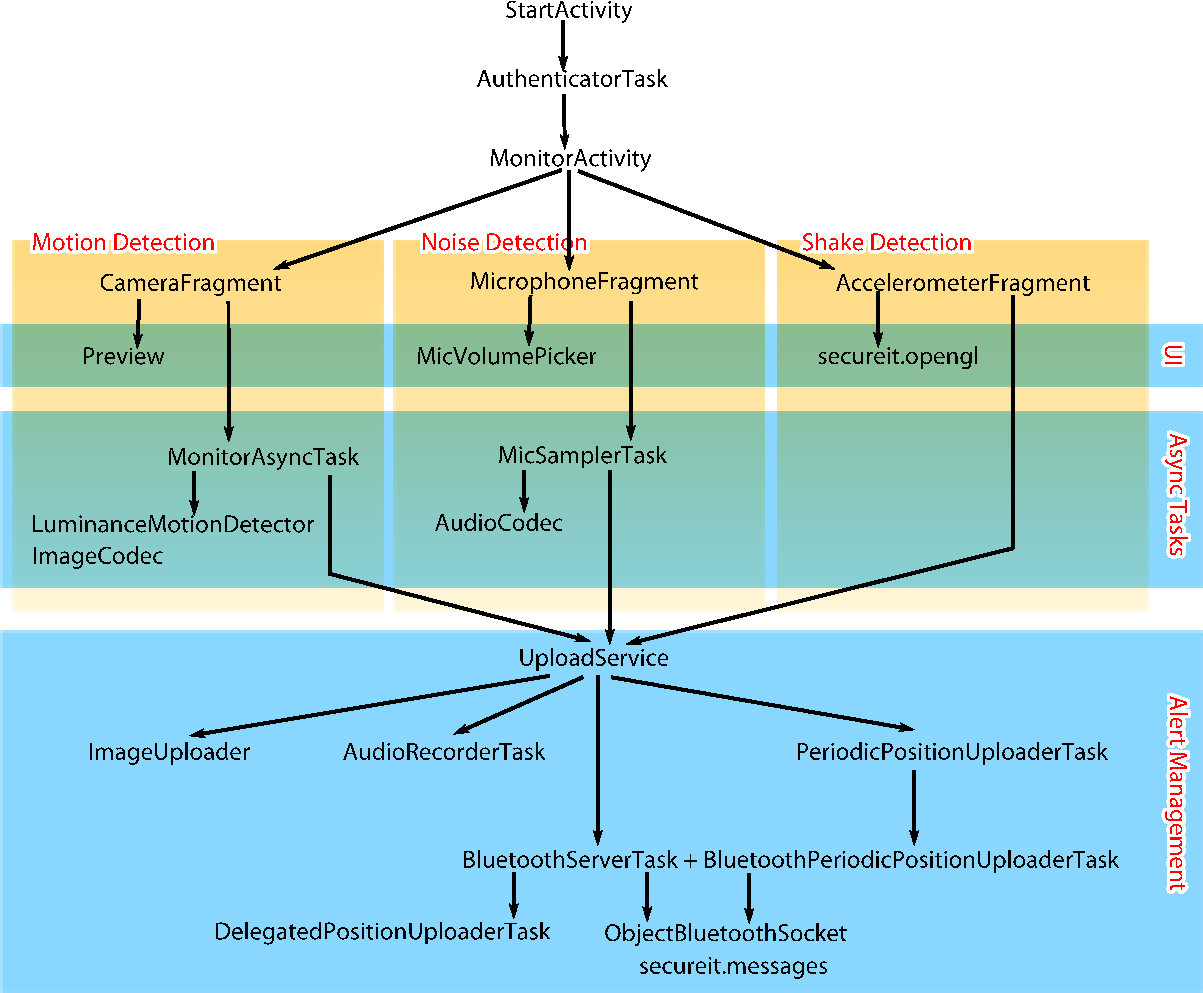
\includegraphics[scale=0.7]{../wireless/resources/architecture.pdf}}
\caption{Diagramma architetturale ad alto livello}
\label{img:architecture}
\end{center}
\end{figure}

Sono state definite tre parti principali che realizzano i computi di monitoraggio dell'applicazione. Ciascuna di queste parti può essere divisa in componenti:

\begin{itemize}
	\item \texttt{Motion Detection}:
		\begin{itemize}
			\item \texttt{CameraFragment}: componente attivo dell'interfaccia grafica visualizzato dall'\texttt{SDK} di Android
			\item \texttt{Preview}: collega l'hardware della fotocamera all'applicativo Java e mostra una superficie contenente i frame catturati
			\item \texttt{MonitorAsyncTask}: elabora i frame catturati per fare motion detection
			\item \texttt{LuminanceMotionDetector}, \texttt{ImageCodec}: classi di utilità per l'analisi dei frame e la conversione di immaginid 
		\end{itemize}
	\item \texttt{Noise Detection}:
		\begin{itemize}
			\item \texttt{MicrophoneFragment}: componente attivo dell'interfaccia grafica visualizzato dall'\texttt{SDK} di Android
			\item \texttt{MicVolumePicker}: vista passiva che mostra il livello sonoro
			\item \texttt{MicSamplerTask}: periodicamente campiona i dati audio utilizzando \texttt{AudioCodec}
			\item \texttt{AudioCodec}: su richiesta campiona l'audio del microfono
		\end{itemize}
	\item \texttt{Motion Detection}:
		\begin{itemize}
			\item \texttt{AccelerometerFragment}: componente attivo dell'interfaccia grafica visualizzato dall'\texttt{SDK} di Android
			\item \texttt{secureit.opengl}: \textit{package} di utilità grafiche per la visualizzazione di animazioni 3D
		\end{itemize}
\end{itemize}

\texttt{UploadService} viene attivato quando uno dei \textit{fragment} identifica un intrusione. Utilizza i seguenti \textit{task} asincroni per realizzare il caricamento dei dati al \textit{back-end}:
\begin{itemize}
	\item \texttt{ImageUploaderTask}: carica le immagini catturate
	\item \texttt{AudioRecorderTask}: registra una traccia audio e la carica
	\item \texttt{PeriodicPositionUploaderTask}: invia periodicamente la posizione del telefono utilizzando rete \texttt{WIFI} o \texttt{3G}
	\item \texttt{Bluetooth\allowbreak Periodic\allowbreak Position\allowbreak Uploader\allowbreak Task}: invia periodicamente la posizione del telefono utilizzando comunication \textit{bluetooth} opportunistica, attivato soltanto non c'è una connessione \texttt{WIFI} o \texttt{3G} attiva
	\item \texttt{BluetoothServerTask}: \textit{task} che risponde a messaggi \textit{bluetooth} e richiede l'\textit{upload} delegato della posizione
	\item \texttt{DelegatedPositionUploaderTask}: invia periodicamente la posizione di un altro telefono su delega
\end{itemize}

Lo scambio di messaggi \textit{bluetooth} viene fatto utilizzando i seguenti moduli:

\begin{itemize}
	\item \texttt{ObjectBluetoothSocket}: \textit{socket} per l'invio di messaggi \textit{bluetooth}
	\item \texttt{secureit.messages}: \textit{package} contenente messaggi \textit{bluetooth}
\end{itemize}


